\section{The Wavelet Gain Layer}

\begin{figure}[t]
  \centering
  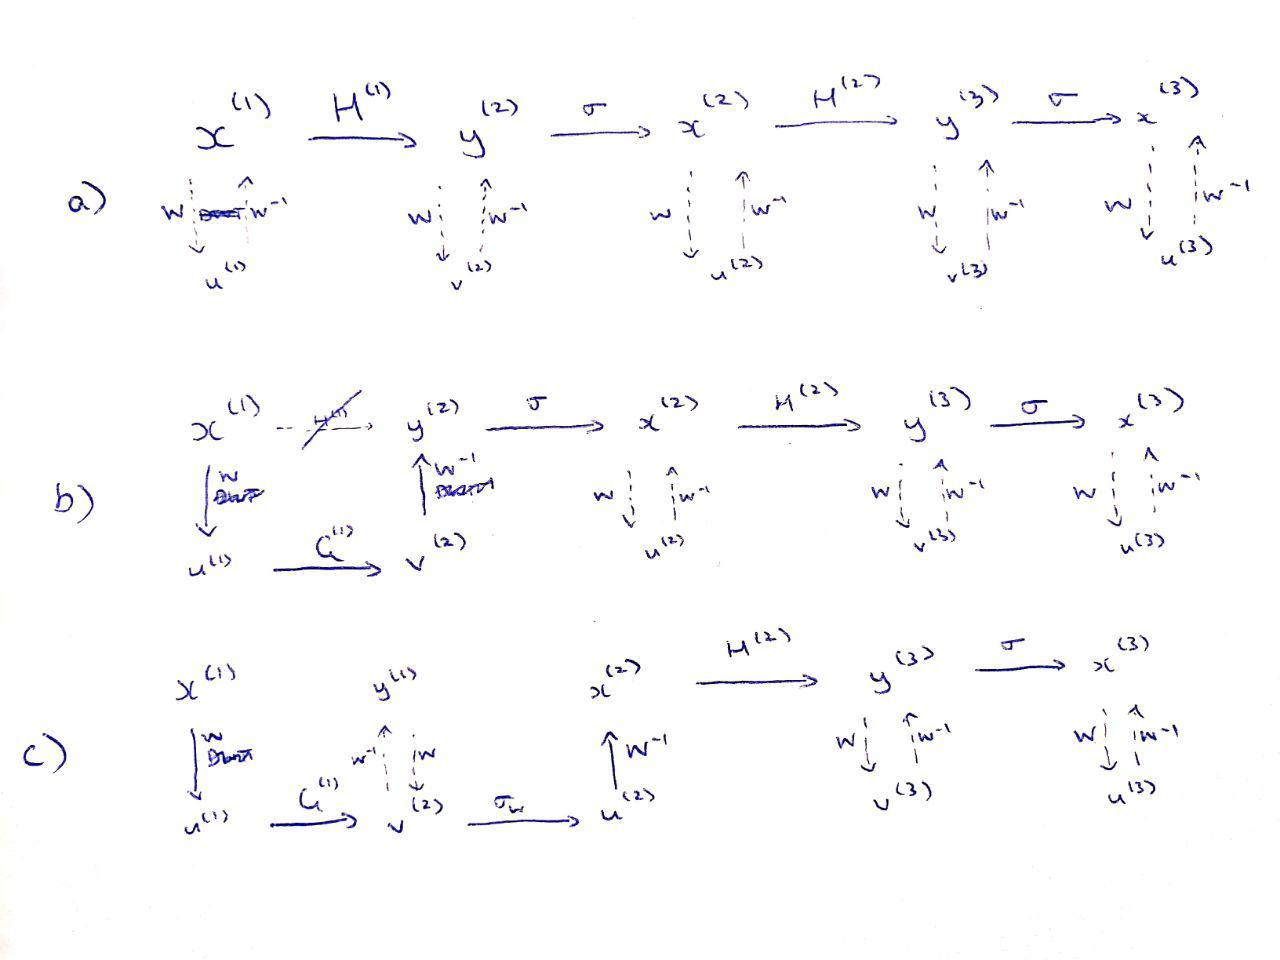
\includegraphics[width=\textwidth]{\imgpath/fwd_chain.jpg}
  \mycaption{Proposed new forward pass in the wavelet domain}{Two network 
  layers with some possible options for processing. Solid lines denote the
  evaluation path and dashed lines indicate relationships. In (a) we see a
  regular convolutional neural network. We have included the dashed lines to
  make clear what we are denoting as $u$ and $v$ with respect to their
  equivalents $x$ and $y$. In (b) we get to $y^{(2)}$ through a different path.
  First we take the wavelet transform of $x^{(1)}$ to give $u^{(1)}$, apply a
  wavelet gain layer $\mathcal{G}^{(1)}$, and take the inverse wavelet transform
  to give $y^{(2)}$. The cross through $\mathcal{H}^{(1)}$ indicates that this
  path is no longer present. Note that there may not be any possible
  $\mathcal{G}^{(1)}$ to make $y^{(2)}$ from (b) equal $y^{(2)}$ from (a). In
  (c) we have stayed in the wavelet domain longer, and applied a wavelet
  nonlinearity $\sigma_w$ to give $u^{(2)}$. We then return to the pixel domain
  to give $x^{(2)}$ and continue on from there in the pixel domain.}
  \label{fig:ch6:fwd_chain}
\end{figure}

At the beginning of each stage of a neural network we have the activations
$x^{(l)}$. Naturally, all of these activations have their equivalent DWT 
coefficients $\mathtt{u}^{(l)}$ and $\DTCWT$ coefficients $u^{(l)}$. 

From \eqref{eq:ch6:conv}, convolutional layers also have intermediate
activations $y^{(l)}$. Let us differentiate these from the $x$ coefficients and
modify \eqref{eq:ch6:dwt_coeffs} and \eqref{eq:ch6:dtcwt_coeffs} to say the DWT
of $y^{(l)}$ gives $\mathtt{v}$ and the $\DTCWT$ of $y^{(l)}$ gives $v$.

We now propose the wavelet gain layers $\mathtt{G}$ and $G$ for the DWT and
$\DTCWT$ respectively, or $\mathcal{G}$ for an implementation agnostic layer.
The name `gain layer' comes from the inspiration for this chapter's work, in
that the first layer of CNN could be nearly done in the wavelet domain by
setting subband gains to 0 and 1. 

The gain layer $\mathcal{G}$ can be used instead of a convolutional layer. 
It is designed to work on the wavelet coefficients of an activation,
$\mathtt{u}$ and $u$ to give outputs $\mathtt{v}$ and $v$. 

This can be seen as breaking the convolutional path in
\autoref{fig:ch6:fwd_chain} and taking a new route to get to the next layer's
coefficients. From here, we can return to the pixel domain by taking the
corresponding inverse wavelet transform $\mathcal{W}^{-1}$. Alternatively, we
can stay in the wavelet domain and apply a wavelet based nonlinearity $\sigma_w$
to give the next layer's $u$ coefficients. Ultimately we would like to explore
architecture design with arbitrary sections in the wavelet and pixel domain, but
to do this we must first explore: 
\begin{itemize}
  \item How effective $\mathcal{G}$ is at replacing $\mathcal{H}$.
  \item How effective $\sigma_w$ is at replcaing $\sigma$.
\end{itemize}

% \subsection{Aliasing in the DWT}
% Consider a single level critically sampled DWT in 1-D. The aliasing cancelling
% condition is:

% $$G_0(z)H_0(-z) + G_1(z)H_1(-z) = 0$$

% This is typically solved by using Quadrature Mirror Filters, i.e.

% \begin{align}
  % H_1(z) &= H_0(-z) \\
  % G_0(z) &= H_0(z) \\
  % G_1(z) &= -H_1(z) = -H_0(-z) 
% \end{align}

\subsection{The DWT Gain Layer}
As mentioned previously, modifying the wavelet coefficients of a critically
sampled DWT will necessarily result in a loss of the aliasing cancelling
properties. However, in a deep neural network, this is not as obviously a bad
thing as it is for denoising or deconvolution. For this reason, we note that
there may be a problem in using a DWT, but proceed nonetheless.

For each subband in our $J$ scale system, we introduce a gain term $\mathtt{g}$. Let us specify our
input $\mathtt{u}$ has $C_l$ channels, and we would like our output $\mathtt{v}$
to have $C_{l+1}$ channels, then $\mathtt{g}$ is made up of:
\begin{eqnarray}
  \mathtt{g}_{lp} &\in& \reals[C_{l+1}\x C_l\x k_h\x k_w] \label{eq:ch6:glp} \\
  \mathtt{g}_{1,1} &\in& \reals[C_{l+1}\x C_l\x k_h\x k_w] \\
  \mathtt{g}_{1,2} &\in& \reals[C_{l+1}\x C_l\x k_h\x k_w] \\
      & \vdots &\\
  g_{J,3} &\in& \reals[C_{l+1}\x C_l\x k_h\x k_w]  \label{eq:ch6:gj3}
\end{eqnarray}
 
\subsection{$\DTCWT$ Multiple Subband Gains}\label{sec:ch6:multiple_subbands}

Now that we have the framework for applying a complex gain at one subband, we
can extend this to all of the subbands in the $\DTCWT$. We also reintroduce the channel
dimension. 

To do the mixing across the $C_l$ channels at each subband, giving $C_{l+1}$
output channels, we introduce the learnable filters:
%
\begin{eqnarray}
  g_{lp} &\in& \reals[C_{l+1}\x C_l\x k_h\x k_w] \label{eq:ch6:glp} \\
  g_{1,1} &\in& \complexes[C_{l+1}\x C_l\x k_h\x k_w] \\
  g_{1,2} &\in& \complexes[C_{l+1}\x C_l\x k_h\x k_w] \\
      & \vdots &\\
  g_{J,6} &\in& \complexes[C_{l+1}\x C_l\x k_h\x k_w]  \label{eq:ch6:gj6}
\end{eqnarray}
%
where $k_h, k_w$ are the sizes of the mixing kernels. These could be $1\x 1$ for
simple gain control, or could be larger, say $3\x 3$, to do more complex
filtering on the subbands. Let us index the lowpass filters $g_{lp}$ and the
bandpass filters $g_{j,k}$ as $g_{lp}[f, c, \nn]$ and $g_{j,k}[f, c, \nn]$.

With these gains we create new coefficients:
\begin{eqnarray}
  v_{lp}[f, \nn] &= & \sum_{c=0}^{C_l-1} u_{lp}[c, \nn] \conv g_{lp}[f, c, \nn] \\
  v_{1,1}[f, \nn] &= & \sum_{c=0}^{C_l-1} u_{1,1}[c, \nn] \conv g_{1,1}[f, c, \nn] \\
  v_{1,2}[f, \nn] &= & \sum_{c=0}^{C_l-1} u_{1,2}[c, \nn] \conv g_{1,2}[f, c, \nn] \\
                  & \vdots & \\
  v_{J,6}[f, \nn] &= & \sum_{c=0}^{C_l-1} u_{J,6}[c, \nn] \conv g_{J,6}[f, c, \nn] 
\end{eqnarray}

I.e., we do independent mixing at each of the different subbands. For $1\x 1$
kernels, this is simply a matrix multiply of the wavelet coefficients. Note that
for complex signals $a, b$ the convolution $a \conv b$ is defined as $(a_r \conv
b_r - a_i \conv b_i) + j(a_r \conv b_i + a_i \conv b_r)$.


\subsection{Examples}
\autoref{fig:ch6:dtcwt_bands} show example impulse responses of our layer.
These impulses were generated by randomly initializing both the real and
imaginary parts of $g_{2,k} \in \complexes[1\x 1]$ from $\mathcal{N}(0,1)$
independently for the six orientations $k$. $g_{1,k}, g_{lp}$ are set to 0. 
I.e. each shape has 12 random variables. It is good
to see that there is still a large degree of variability between shapes. Our
experiments have shown that the distribution of the normalized cross-correlation
between 512 of such randomly generated shapes matches the distribution for
random vectors with roughly 11.5 degrees of freedom.
\autoref{fig:ch6:dtcwt_bands} shows the frequency support of the $6J+1$ subbands
for a two scale $\DTCWT$ as well as some of the equivalent impulse responses for
a randomly initialized set of $g$ filters.

\begin{tikzpicture}[%
  path image/.style={
    path picture={
      \node at (path picture bounding box.center) {
        \includegraphics[height=2.0cm]{#1}
      };
    }
  }, 
  path pic/.style={
    path picture={
      \node at (path picture bounding box.center) {
        \includegraphics[height=1.2cm]{#1}
      };
    }
  }, 
  path pic2/.style={
    path picture={
      \node at (path picture bounding box.center) {
        \includegraphics[height=0.8cm]{#1}
      };
    }
  }, 
  scale=0.6]

  \tikzcuboid{
  shiftx=-1.5cm,
  shifty=-2.5cm,
  scale=0.5,
  anglex=0, 
  angley=90, 
  anglez=230,
  dimx=3, 
  dimy=3, 
  dimz=6,
  densityx=1, 
  densityy=1, 
  densityz=1,
  shade=false,
  emphedge=true,
  shadeopacity=0,
  emphstyle/.style={rounded corners=0.2pt,line width=0.3mm},
  front/.style={draw=blue!50!white,fill=blue!50!white},%
  right/.style={draw=blue!50!white,fill=blue!50!white},%
  top/.style={draw=blue!50!white,fill=blue!50!white},%
  drawxdims=true,
  dimxval=W,
  drawydims=true,
  dimyval=H,
  drawzdims=true,
  dimzval=C_l,
  }
  \draw (0, .3, 0) node {\large{$x^{(l)}$}};
  \draw [path image=\imgpath/waveys.png, draw=black] (1.5,1.5,0) rectangle (6,0,0);
  \draw (3.75, 1.9, 0) node {\large{$\psi_{j, \theta}$}};
  \draw (1.5,0,0) -- (3,-1.7,0);
  \draw (6,0,0) -- (3.3,-1.7,0);
  \draw [path pic2=\imgpath/lowpass.png, draw=black] (2.5,-2.5,10) rectangle (3.5,-1.5,10);
  \draw (3, -1.1, 10) node {\large{$\phi_{j}$}};
  \draw (3.5,-1.5,10) -- (3.5,-1.7,8);

  % \draw (2.4, -1.5, 0) node {\Large{$\conv$}};
  \draw (2.5, -1.5, 3) node {\Large{$\conv$}};
  \draw [->, fill=gray!30,ultra thick] (4, -1.5, 0) -- (5, -1.5, 0);
  \draw [->, fill=gray!30,ultra thick] (4.5, -1.5, 9) -- (5.85, -1.5, 11);

  \tikzcuboid{
  shiftx=3cm,
  shifty=-1.7cm,
  shiftz=0,
  scale=0.3,
  dimx=1, dimy=1, dimz=4,
  densityx=2, densityy=2, densityz=2,
  drawxdims=false,
  drawydims=false,
  drawzdims=true,
  dimzval=12,
  front/.style={draw=yellow!70!white,fill=yellow!70!white},%
  right/.style={draw=yellow!70!white,fill=yellow!70!white},%
  top/.style={draw=yellow!70!white,fill=yellow!70!white},%
  }
  \tikzcuboid{
  shiftz=8/0.3,
  scale=0.3,
  dimx=1, dimy=1, dimz=1,
  densityx=2, densityy=2, densityz=2,
  drawxdims=false,
  drawydims=false,
  drawzdims=false,
  }


  \tikzcuboid{
  shiftx=6cm,
  shifty=-2.0cm,
  shiftz=0.8cm,
  scale=0.5,
  dimx=2, dimy=2, dimz=4,
  densityx=4, densityy=4, densityz=2,
  drawzdims=true,
  dimzval=C_l,
  front/.style={draw=blue!50!white,fill=blue!50!white},%
  right/.style={draw=blue!50!white,fill=blue!50!white},%
  top/.style={draw=blue!50!white,fill=blue!50!white},%
  }

  \tikzcuboid{
  shiftx=6cm,
  shifty=-2cm,
  shiftz=0cm,
  scale=0.5,
  dimx=2, dimy=2, dimz=24,
  densityx=2, densityy=2, densityz=2,
  drawxdims=true,
  dimxval=\frac{W}{2},
  drawydims=true,
  dimyval=\frac{H}{2},
  drawzdims=true,
  dimzval=12C_l,
  front/.style={draw=blue!50!white,fill=blue!50!white},%
  right/.style={draw=blue!50!white,fill=blue!50!white},%
  top/.style={draw=blue!50!white,fill=blue!50!white},%
  }

  % \draw [->, fill=gray!30,ultra thick] (8.5, -1.5, 0) -- (10.5, -1.5, 0) node[midway, above] (mag) {\large{$\lvert\cdot\rvert$}};
  \draw [->, fill=gray!30,ultra thick] (8.5, -1.5, 0) -- (10.5, -1.5, 0) node[midway, above] (mag) {\Large{ $\lvert \cdot \rvert$} };
  \draw [path pic=\imgpath/mag.png, draw=white] (9.25,0,0) rectangle (11.75,2,0);
  \draw (9.25,0,0) -- (mag.north);
  \draw (11.75,0,0) -- (mag.north);
  \draw[->, fill=gray!30, ultra thick] (8.5, -2, 10) -- (10, -3, 3);

  \tikzcuboid{
  shiftx=11.5cm,
  shifty=-2cm,
  scale=0.5,
  dimx=2, dimy=2, dimz=12,
  densityx=2, densityy=2, densityz=2,
  dimzval=6C_l,
  drawxdims=false,
  drawydims=false,
  front/.style={draw=blue!50!white,fill=blue!50!white},%
  right/.style={draw=blue!50!white,fill=blue!50!white},%
  top/.style={draw=blue!50!white,fill=blue!50!white},%
  }
  \tikzcuboid{
  shiftx=11.5cm,
  shifty=-2cm,
  shiftz=8,
  scale=0.5,
  drawxdims=true,
  drawydims=true,
  dimx=2, dimy=2, dimz=4,
  densityx=2, densityy=2, densityz=2,
  dimzval=C_l,
  front/.style={draw=blue!50!white,fill=blue!50!white},%
  right/.style={draw=blue!50!white,fill=blue!50!white},%
  top/.style={draw=blue!50!white,fill=blue!50!white},%
  }
  \draw (13.2, 0.8, 0) node {\large{$z^{(l+1)}$}};
  \draw (20.5, 0.3, 0) node {\large{$y^{(l+1)}$}};
  \draw (24.5, 0.3, 0) node {\large{$x^{(l+1)}$}};
  \draw (14, -1.5, 0) node {\Large{$\conv$}};

  \tikzcuboid{
  shiftx=15.2cm,
  shifty=-1.0cm,
  shiftz=0,
  scale=0.5,
  dimx=0.4, dimy=0.4, dimz=14,
  densityx=5, densityy=5, densityz=2,
  drawxdims=false,
  drawydims=false,
  drawzdims=false,
  front/.style={draw=red!50!white,fill=red!50!white},%
  right/.style={draw=red!50!white,fill=red!50!white},%
  top/.style={draw=red!50!white,fill=red!50!white},%
  }
  \tikzcuboid{
  shifty=-1.65cm,
  }
  \tikzcuboid{
  shifty=-3.0cm,
  scale=0.5,
  drawxdims=true,
  dimxval=1,
  drawydims=true,
  dimyval=1,
  drawzdims=true,
  dimzval=7C_l,
  }
  \draw (15.5, -1.8, 0) node {$\vdots$};
  \draw [<->] (15.7, -0.8, -3) -- (15.7, -3, -3) node[near start, right] {$C_{l+1}$};
  \draw [->, fill=gray!30,ultra thick] (17.5, -1.5, 0) -- (18.5, -1.5, 0);

  \tikzcuboid{
  shiftx=19.5cm,
  shifty=-2.25cm,
  scale=0.5,
  dimx=2, dimy=2, dimz=6,
  densityx=4, densityy=4, densityz=2,
  drawzdims=false,
  drawxdims=false,
  drawydims=false,
  front/.style={draw=blue!50!white,fill=blue!50!white},%
  right/.style={draw=blue!50!white,fill=blue!50!white},%
  top/.style={draw=blue!50!white,fill=blue!50!white},%
  }
  \draw [->, fill=gray!30,ultra thick] (21.5, -1.5, 0) -- (22.5, -1.5, 0)
    node[midway, above] {$\sigma$};

  \tikzcuboid{
  shiftx=23.5cm,
  shifty=-2.25cm,
  scale=0.5,
  dimx=2, dimy=2, dimz=6,
  densityx=4, densityy=4, densityz=2,
  drawzdims=true,
  dimzval=C_{l+1},
  drawxdims=true,
  dimxval=\frac{W}{2},
  drawydims=true,
  dimyval=\frac{H}{2},
  front/.style={draw=blue!50!white,fill=blue!50!white},%
  right/.style={draw=blue!50!white,fill=blue!50!white},%
  top/.style={draw=blue!50!white,fill=blue!50!white},%
  }

\end{tikzpicture}


